% Proton therapy presentation for funding evaluation.
% Compile: latexmk -pdf pbt_argos.tex
\documentclass[aspectratio=169,11pt]{beamer}

\usepackage[T1]{fontenc}
\usepackage[utf8]{inputenc}
\usepackage{helvet}
\usepackage{graphicx}
\usepackage{booktabs}
\usepackage{array}
\usepackage{amsmath}
\usepackage{tikz}
\usepackage{eurosym}
\usetikzlibrary{shapes.geometric, arrows.meta, positioning, backgrounds}

\graphicspath{{figs/}}

% ---- clean custom look (no external theme needed) --------------------------
\usetheme{default}
\setbeamertemplate{navigation symbols}{}
\definecolor{crBlue}{RGB}{22,88,138}
\definecolor{crRed}{RGB}{200,74,40}
\definecolor{crGrey}{RGB}{90,95,100}
\setbeamercolor{title}{fg=crBlue}
\setbeamercolor{frametitle}{fg=crBlue}
\setbeamercolor{structure}{fg=crBlue}
\setbeamercolor{normal text}{fg=black}
\setbeamerfont{frametitle}{series=\bfseries, size=\large}
\setbeamerfont{title}{series=\bfseries}
\setbeamertemplate{itemize item}{\color{crRed}\textbullet}
\setbeamertemplate{itemize subitem}{\color{crGrey}--}
\setbeamertemplate{frametitle}{%
  \vspace{3mm}\hspace{2mm}%
  {\usebeamerfont{frametitle}\usebeamercolor[fg]{frametitle}\insertframetitle}\par
  {\color{crBlue}\rule{\textwidth}{1.1pt}}\vspace{-1mm}}
\setbeamertemplate{footline}{%
  \hbox{}\hfill{\color{crGrey}\scriptsize\insertframenumber\,/\,\inserttotalframenumber}%
  \hspace{3mm}\vspace{2mm}}

\newcommand{\OT}{\textsuperscript{15}O}
\newcommand{\CE}{\textsuperscript{11}C}
\newcommand{\hi}[1]{\textcolor{crRed}{#1}}


\setbeamersize{text margin left=7mm,text margin right=7mm}
\newcommand{\source}[2]{\par\vspace{2mm}{\tiny\color{crGrey}\href{#1}{#2}\par}}
\title{Boosting proton beam therapy potential}
\subtitle{Clinical motivation and measurement principles}
\author{DIPC CRYSP group}
\date{\small Working draft --- \today}
\begin{document}
{\setbeamertemplate{footline}{}
\begin{frame}[plain,noframenumbering]
\titlepage
\end{frame}}
\begin{frame}{What is proton therapy?}
  \small
  \begin{columns}[T]
    \begin{column}{0.52\textwidth}
      \begin{itemize}
        \item A form of \hi{external-beam radiotherapy} that uses
          accelerated protons to destroy tumour cells.
        \item Protons are \hi{positively charged particles}:
          their energy determines how deep they travel in tissue.
        \item Their dose peaks near the end of their range
          (the \hi{Bragg peak}), then falls sharply.
        \item Combining different proton energies covers the tumour
          volume, while \hi{reducing dose beyond it} compared with X-rays.
      \end{itemize}
    \end{column}
    \begin{column}{0.48\textwidth}
      \centering
      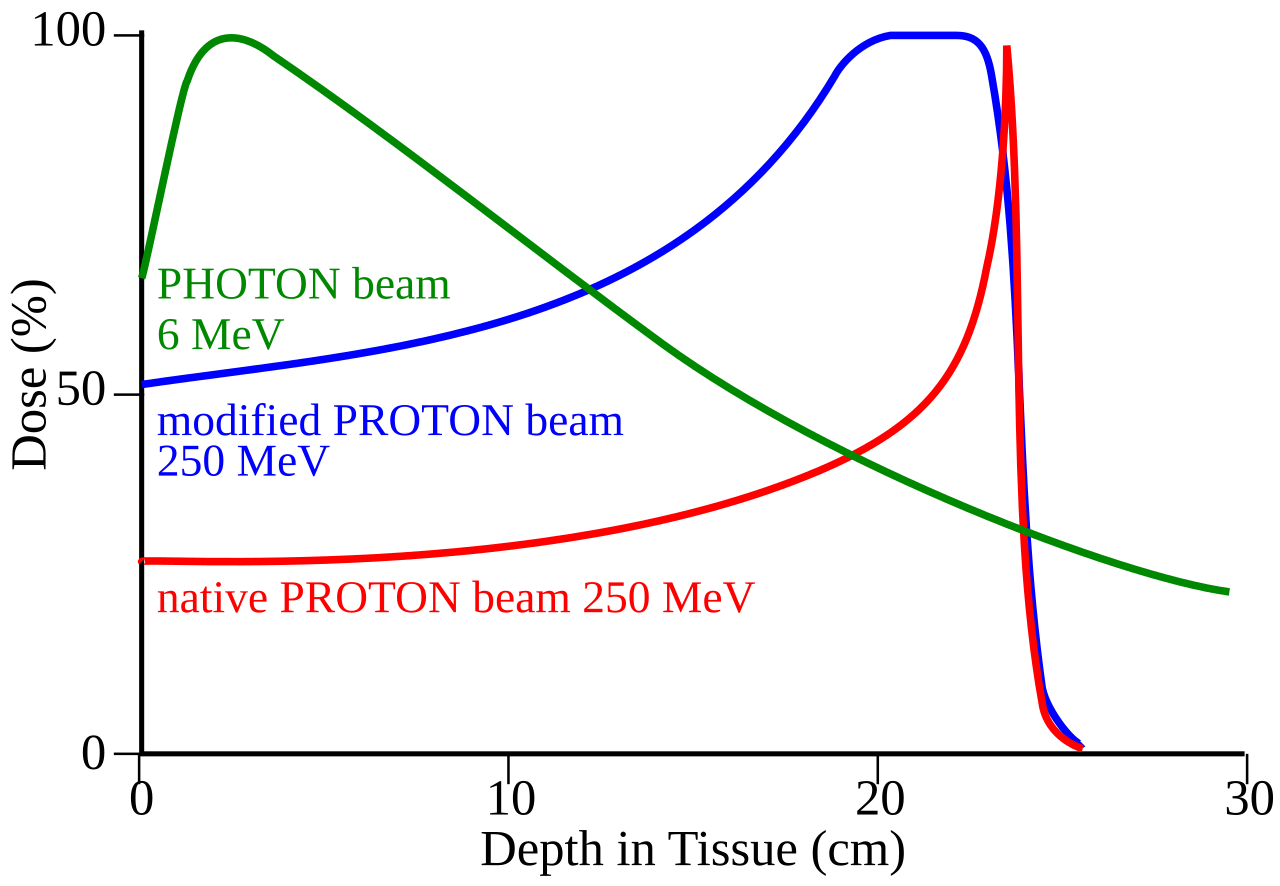
\includegraphics[width=\linewidth]{proton_therapy_bragg.png}\\[1mm]
      {\scriptsize\color{crGrey} Schematic depth--dose profiles: a single
       proton energy, a spread-out peak and an X-ray beam.}\\[2mm]
      {\tiny\color{crGrey}
       \href{https://commons.wikimedia.org/wiki/File:BraggPeak-en.svg}
       {Image: D. Ilyin / A. A. Miller, Wikimedia Commons (CC0).}\\
       \href{https://www.cancer.gov/about-cancer/treatment/types/radiation-therapy/external-beam}
       {Reference: National Cancer Institute, External Beam Radiation Therapy.}}
    \end{column}
  \end{columns}
\end{frame}


\begin{frame}{Example: Brain tumours}
\small
\begin{columns}[T,onlytextwidth]
\begin{column}{0.57\textwidth}
\begin{itemize}
\item Brain and CNS tumours are the \hi{most common solid tumours in children}: about \hi{300 new cases a year in Spain}.
\item In adults, malignant brain/CNS tumours account for roughly \hi{4,400 cases a year in Spain} (about 1.5\% of cancers).
\item Childhood ependymomas often arise near the \hi{cerebellum and brainstem}. The goal is to cover the tumour while sparing these structures.
\end{itemize}
\source{https://www.pediatriaintegral.es/publicacion-2021-10/tumores-cerebrales-en-ninos-2021/}{Childhood estimate: Pediatr\'ia Integral (2021), based on RETI.}
\source{https://redecan.org/storage/documents/dc9dc273-8b61-475f-ae4f-88d447dc81fc.pdf}{Adult figure: approximate, from REDECAN 2026 all-age malignant CNS estimate.}
\end{column}
\begin{column}{0.39\textwidth}
\centering
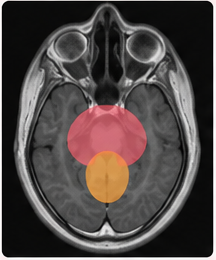
\includegraphics[height=0.34\textheight]{argos_brain_skullbase.png}\\[1mm]
{\scriptsize Brain/skull-base example: tumour (pink), brainstem (orange).}
\par\vspace{3mm}
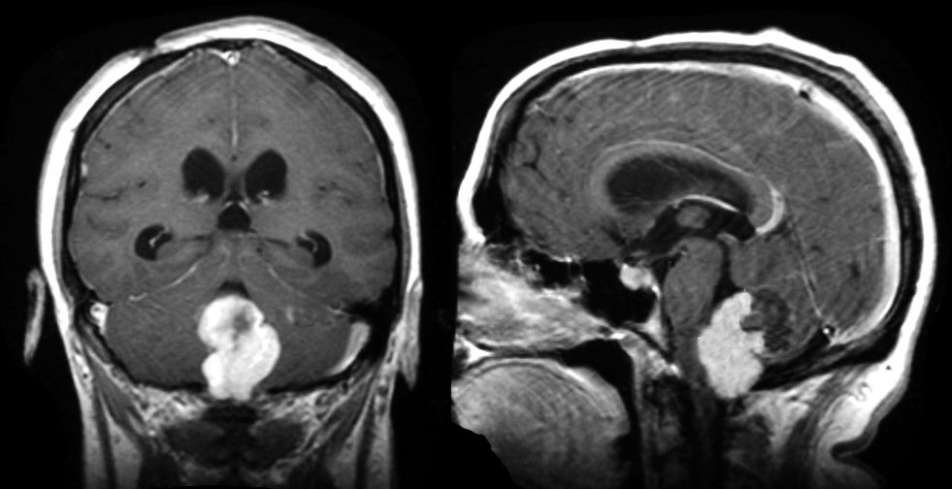
\includegraphics[width=0.78\linewidth,height=0.16\textheight,keepaspectratio]{ependymoma_mri.png}\\
{\scriptsize Fourth-ventricle ependymoma (MRI).}
\end{column}
\end{columns}
\end{frame}



\begin{frame}{From treatment planning to delivery}
\small
\centering
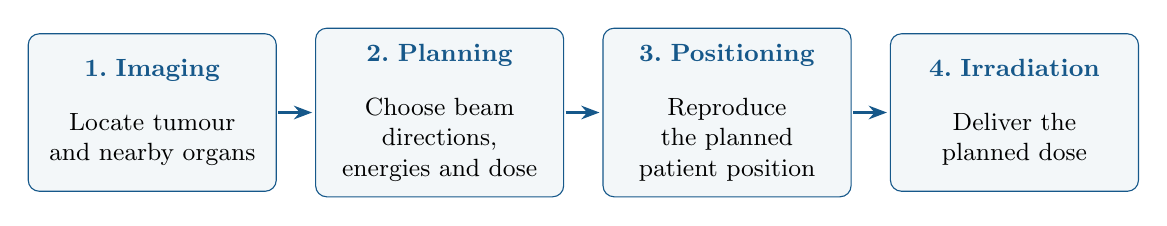
\begin{tikzpicture}[font=\small,>=Stealth]
\foreach \x/\num/\heading/\body in {0/1/Imaging/{Locate tumour\\and nearby organs},3.65/2/Planning/{Choose beam directions,\\energies and dose},7.3/3/Positioning/{Reproduce the planned\\patient position},10.95/4/Irradiation/{Deliver the\\planned dose}} {
\node[draw=crBlue,fill=crBlue!5,rounded corners,text width=2.75cm,inner sep=2mm,minimum width=3.15cm,minimum height=2cm,align=center] at (\x,0) {\textcolor{crBlue}{\textbf{\num.\ \heading}}\\[3mm]\body};}
\foreach \x in {1.60,5.25,8.90} {\draw[->,thick,crBlue] (\x,0)-- +(0.43,0);}
\end{tikzpicture}
\par\vspace{3mm}
\begin{columns}[T,onlytextwidth]
\begin{column}{0.48\textwidth}
\textbf{Delivered dose can differ from plan}
\begin{itemize}
\item Uncertainty in tissue stopping power.
\item Anatomical changes, positioning and motion.
\end{itemize}
\end{column}
\begin{column}{0.48\textwidth}
\textbf{Unlike photons, protons are absorbed in the patient's body}
\par\vspace{3mm}
The plan delivers a \hi{prediction} of proton range. \hi{How to check it?}
\end{column}
\end{columns}
\end{frame}



\begin{frame}{Why range uncertainty matters}
\small
\centering
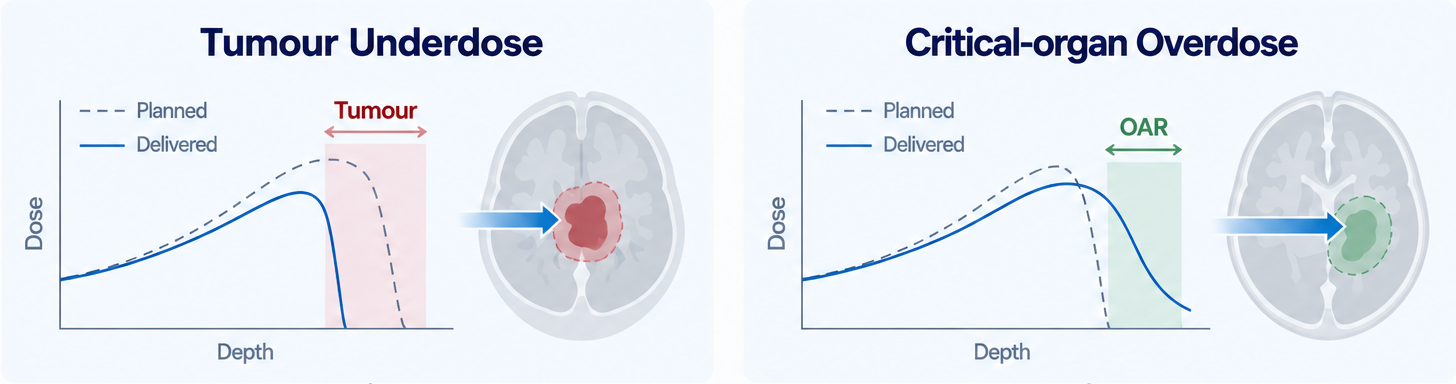
\includegraphics[width=0.92\textwidth,height=0.31\textheight,keepaspectratio]{argos_range_errors.png}
\par\vspace{3mm}
\begin{columns}[T,onlytextwidth]
\begin{column}{0.60\textwidth}
\begin{itemize}
\item Systematic errors in proton range \hi{estimation} are of the order of \hi{3.5\%}.
\item The required planning margins are of the order of several mm.
\item Conservative beam choices protect nearby organs, but can limit coverage when tumour and organ are close.
\end{itemize}
\end{column}
\begin{column}{0.36\textwidth}
\centering
\textbf{Example at 10\,cm depth}\\[3mm]
\hi{$0.035\times100\,\mathrm{mm}+1\,\mathrm{mm}$}\\[2mm]
\hi{$=4.5\,\mathrm{mm}$}\\[3mm]
{\scriptsize 3.5\% range allowance plus 1\,mm.\\Margins depend on the centre and treatment site.}
\end{column}
\end{columns}
\source{https://doi.org/10.1088/0031-9155/57/11/R99}{Range uncertainty: Paganetti, Phys. Med. Biol. 57, R99 (2012). OAR = organ at risk.}
\end{frame}



\begin{frame}{What could better range verification change?}
\small
\begin{columns}[T,onlytextwidth]
\begin{column}{0.53\textwidth}
\begin{itemize}
\item With less range uncertainty, planners can reduce dose to \hi{healthy tissue near the tumour}.
\item They may also use \hi{beam directions otherwise avoided} because a critical organ lies near the stopping point.
\item Verification must show that the uncertainty is sufficiently small before these changes can be adopted.
\end{itemize}
\end{column}
\begin{column}{0.43\textwidth}
\begin{beamercolorbox}[sep=3mm,wd=\linewidth]{block body}
\textbf{A planning study: 27 brain-tumour patients}
\par\vspace{3mm}
Range uncertainty reduced from \hi{3\% to 2\%}.
\par\vspace{3mm}
\hi{24 of 27 patients (89\%)} had a relevant dose reduction to at least one organ at risk.
\end{beamercolorbox}
\end{column}
\end{columns}
\par\vspace{3mm}
In brain tumours, proton range uncertainties of \hi{1\,mm or less} can in principle be achieved.$^{*}$
\source{https://doi.org/10.1259/bjr.20230110}{Taasti et al., British Journal of Radiology 96, 20230110 (2023).}
\source{https://doi.org/10.1002/mp.15644}{Beam-direction benefit: Tattenberg et al., Medical Physics (2022).}
\par\vspace{1mm}{\scriptsize\color{crGrey}$^{*}$J.J. G\'omez-Cadenas et al., \emph{A High-Sensitivity In-Room CRYSP Scanner for Distal-Edge Verification in Proton Therapy}, paper in preparation, available upon request.}
\end{frame}


\begin{frame}{Complementary imaging for proton therapy}
\small
\begin{columns}[T,onlytextwidth]
\begin{column}{0.48\textwidth}
\centering
\textbf{Compton camera}\\
In-beam: prompt $\gamma$ rays
\par\vspace{1mm}
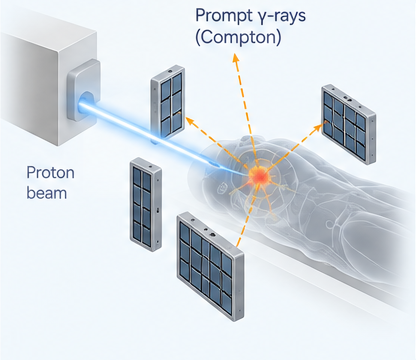
\includegraphics[height=0.40\textheight,keepaspectratio]{argos_compton_illustration.png}
\end{column}
\begin{column}{0.48\textwidth}
\centering
\textbf{PET}\\
In-room, post-treatment: $\beta^+$ activity
\par\vspace{1mm}
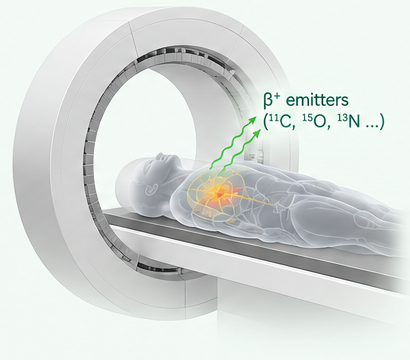
\includegraphics[height=0.40\textheight,keepaspectratio]{argos_pet_illustration.png}
\end{column}
\end{columns}
\par\vspace{2mm}
R\&D studies support Compton cameras and PET for \hi{proton range verification}. No dedicated commercial solution identified.
\par\vspace{2mm}
% References transcribed from ARGOS slide 12; bibliographic details need verification.
\begin{columns}[T,onlytextwidth]
\begin{column}{0.48\textwidth}
{\scriptsize\color{crGrey}
Safavi et al., Nat. Commun. 17, 206 (2026).\par\vspace{1mm}
Sharma et al., Med. Phys. 52, 1123 (2025).}
\end{column}
\begin{column}{0.48\textwidth}
{\scriptsize\color{crGrey}
Parodi et al., Eur. J. Nucl. Med. Mol. Imaging 51, 183 (2024).\par\vspace{1mm}
Zhu et al., Phys. Med. Biol. 56, 6425 (2011).}
\end{column}
\end{columns}
\end{frame}

\begin{frame}{PET: an \emph{in vivo} probe of where the beam stopped}
  \small
  \begin{columns}[T]
    \begin{column}{0.54\textwidth}
      \begin{itemize}
        \item Above the nuclear-reaction threshold, protons create
          \hi{$\beta^+$ emitters} along their path --- mainly \OT\ and \CE.
        \item Their annihilation $\gamma$'s are imaged in coincidence: a PET
          image of the \hi{induced activity}.
        \item The activity falloff sits just upstream of the dose edge; its
          \hi{distal edge tracks the range}.
      \end{itemize}
    \end{column}
    \begin{column}{0.46\textwidth}
      \centering
      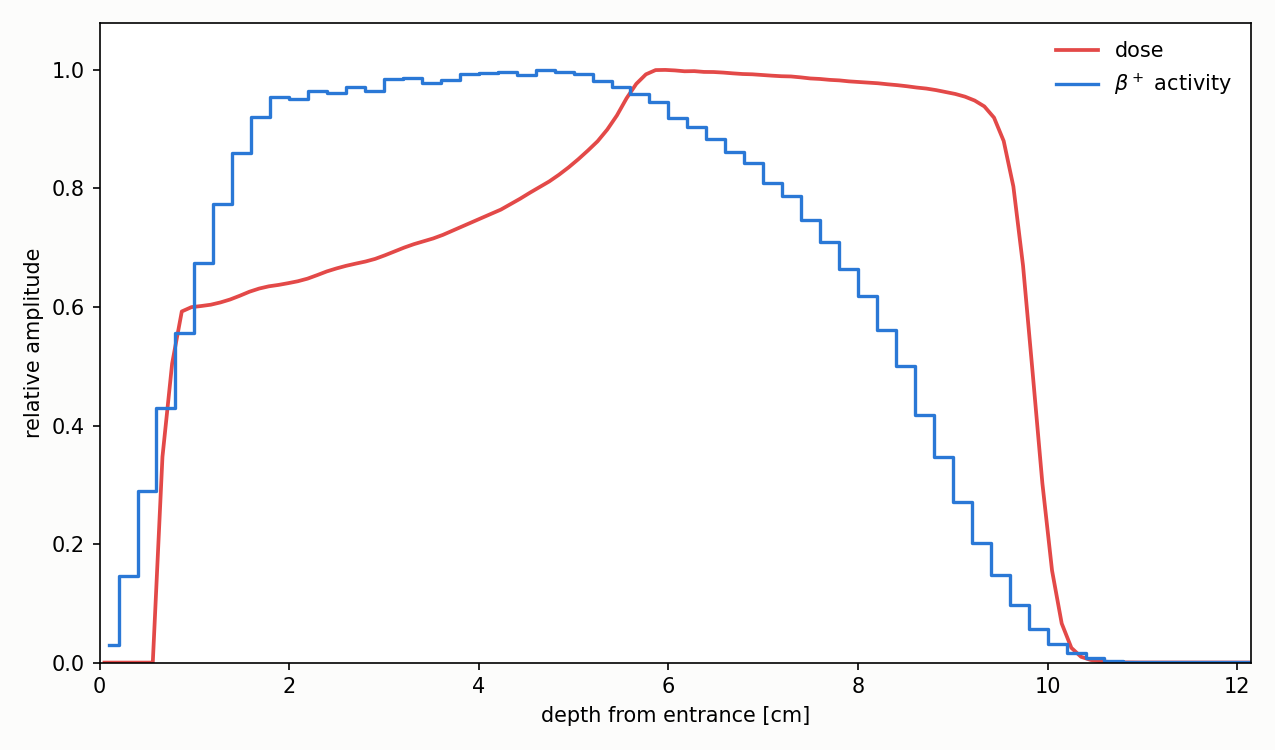
\includegraphics[width=\linewidth]{dose_activity.png}\\
      {\scriptsize\color{crGrey} Illustrative dose and $\beta^+$ activity profiles.\\[2mm]
       The activity edge is compared with a prediction to estimate the range.}
    \end{column}
  \end{columns}
\end{frame}

\begin{frame}{PET range verification: offline, in-beam and in-room}
  \centering
  
\includegraphics[width=0.94\textwidth,height=0.80\textheight,keepaspectratio]{in-room.png}
\end{frame}

\begin{frame}{PET range verification: offline, in-beam and in-room}
  \centering
  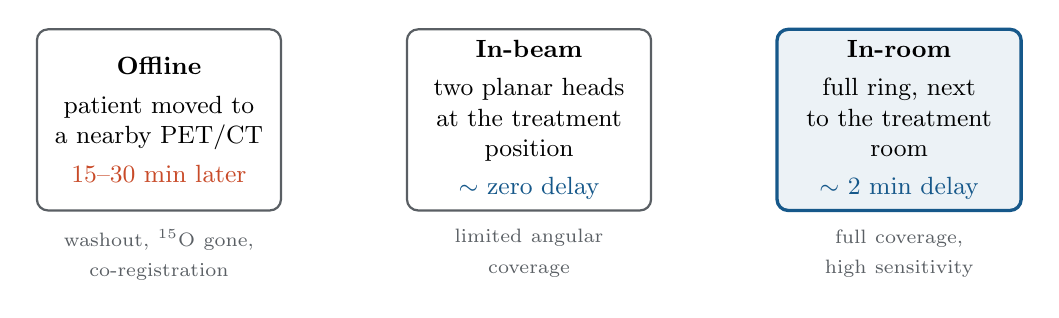
\begin{tikzpicture}[font=\small, node distance=6mm]
    % offline
    \node[draw=crGrey, rounded corners, minimum width=3.1cm, minimum height=2.3cm,
          align=center, thick] (off) at (0,0)
      {\textbf{Offline}\\[1mm] patient moved to\\ a nearby PET/CT\\[1mm]
       \textcolor{crRed}{15--30 min later}};
    % in-beam
    \node[draw=crGrey, rounded corners, minimum width=3.1cm, minimum height=2.3cm,
          align=center, thick] (ib) at (4.7,0)
      {\textbf{In-beam}\\[1mm] two planar heads\\ at the treatment\\ position\\[1mm]
       \textcolor{crBlue}{$\sim$ zero delay}};
    % in-room
    \node[draw=crBlue, fill=crBlue!8, rounded corners, minimum width=3.1cm,
          minimum height=2.3cm, align=center, very thick] (ir) at (9.4,0)
      {\textbf{In-room}\\[1mm] full ring, next\\ to the treatment\\ room\\[1mm]
       \textcolor{crBlue}{$\sim$ 2 min delay}};
    \node[below=1mm of off, text width=3.1cm, align=center, crGrey]
      {\scriptsize washout, \OT\ gone,\\ co-registration};
    \node[below=1mm of ib, text width=3.1cm, align=center, crGrey]
      {\scriptsize limited angular\\ coverage};
    \node[below=1mm of ir, text width=3.1cm, align=center, crGrey]
      {\scriptsize full coverage,\\ high sensitivity};
  \end{tikzpicture}
  \vspace{2mm}

  {\color{crGrey}\small The trade-off is \textbf{delay} vs.\ \textbf{angular
   coverage / scanner quality}.}
\end{frame}

\begin{frame}{Offline results in large uncertainties}
  \begin{columns}[T]
    \begin{column}{0.56\textwidth}
      A delay of 15--30 minutes costs on three fronts:
      \begin{itemize}
        \item \hi{Sensitivity}: the abundant \OT\ (2\,min) has vanished --- only
          the sparse \CE\ tail remains.
        \item \hi{Biological washout}: perfusion clears the emitters; hard to
          model, patient-dependent.
        \item \hi{Co-registration}: the patient is set up afresh on a separate
          scanner --- a few-mm misalignment maps straight into an apparent
          range shift.
      \end{itemize}
      \vspace{1mm}
%      {\small\color{crGrey} Literature: offline accuracy a few mm at best
%       (Knopf 2009; Parodi).}
    \end{column}
    \begin{column}{0.44\textwidth}
      \centering
      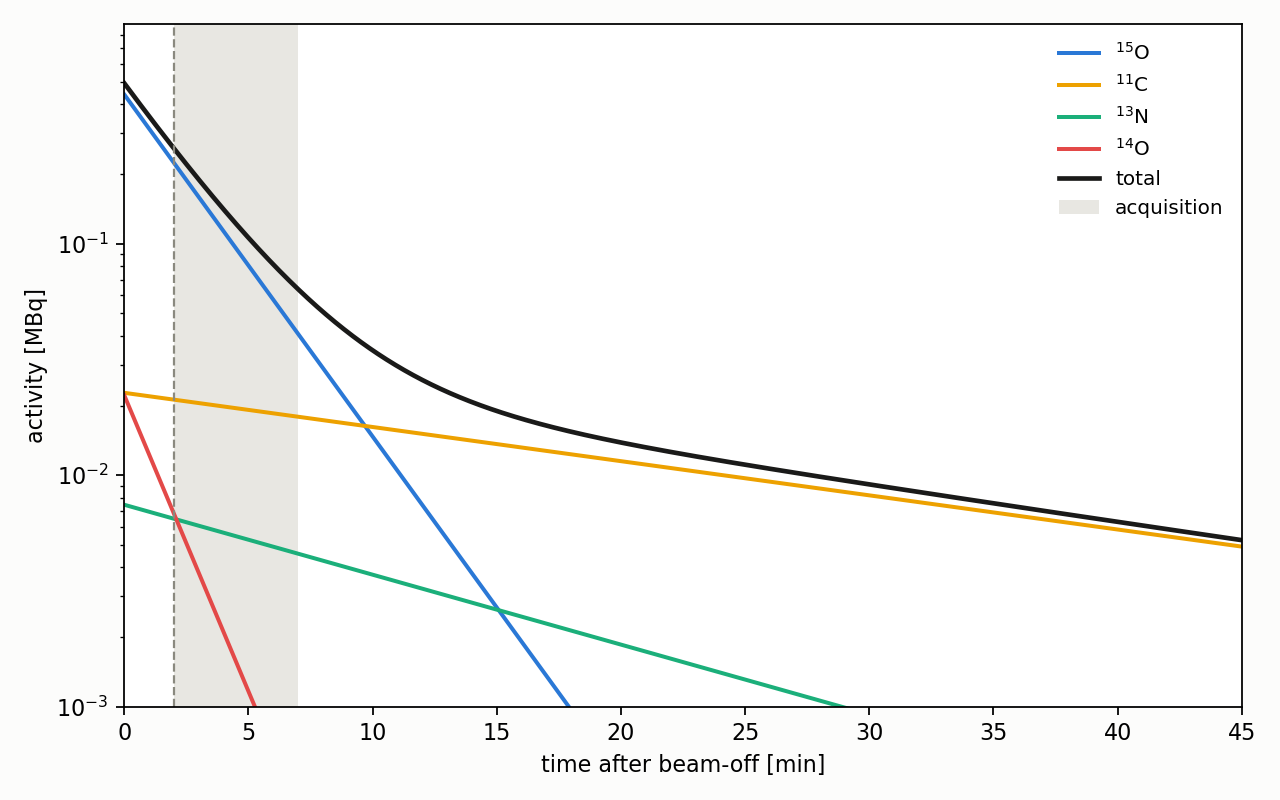
\includegraphics[width=\linewidth]{activity.png}\\
      {\scriptsize\color{crGrey} \OT\ dominates the first minutes, then decays;
       \CE\ carries the late, weak signal.}
    \end{column}
  \end{columns}
\end{frame}

\begin{frame}{Online/In-room tradeoffs}
  \begin{columns}[T]
    \begin{column}{0.5\textwidth}
      \textbf{\color{crBlue}In-beam} (short delay, same bed)
      \begin{itemize}
        \item Retains the short-lived \OT, essentially no delay.
        \item But the beam must pass: only \hi{two planar heads} fit.
        \item Reduced angular coverage $\Rightarrow$ \hi{low sensitivity} and
          limited-angle image artefacts.
      \end{itemize}
    \end{column}
    \begin{column}{0.5\textwidth}
      \textbf{\color{crBlue}In-room} (just after, full ring)
      \begin{itemize}
        \item A \hi{full closed ring} $\Rightarrow$ full coverage, high
          sensitivity, clean image.
        \item Same couch $\Rightarrow$ a known rigid transform and a short
          transfer, without separate-scanner repositioning.
        \item The $\sim$2-min delay is \hi{bought back} by sensitivity and a
          \hi{better scanner}.
      \end{itemize}
    \end{column}
  \end{columns}
  \vspace{2mm}
  \begin{center}
    \fbox{\parbox{0.9\textwidth}{\centering
      A \hi{high-sensitivity in-room ring} combines short transfer time with
      complete angular coverage and high sensitivity.}}
  \end{center}
\end{frame}

% ===========================================================================

\begin{frame}{Prompt gammas: tracking the proton range during irradiation}
  \small
  \begin{columns}[T]
    \begin{column}{0.54\textwidth}
      \begin{itemize}
        \item Nuclear reactions along the proton path leave excited nuclei
          in the tissue. Their de-excitation emits \hi{prompt $\gamma$ rays}
          with energies of several MeV.
        \item Emission occurs \hi{during irradiation}. Its distal falloff
          tracks the proton range; the relation depends on tissue
          composition and the selected $\gamma$ energies.
        \item The measured \hi{4.4\,MeV $\gamma$ profile} shown here
          concentrates near the Bragg peak and follows the proton range.
      \end{itemize}
    \end{column}
    \begin{column}{0.46\textwidth}
      \centering
      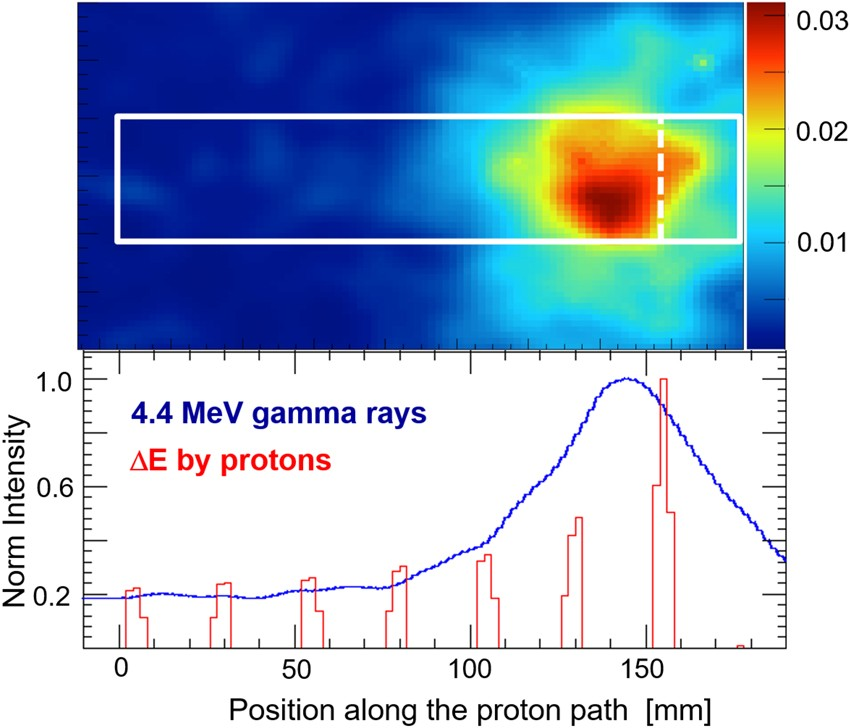
\includegraphics[width=\linewidth,height=0.53\textheight,keepaspectratio]
        {prompt_gamma_compton_koide2018.jpg}\\[1mm]
      {\scriptsize\color{crGrey} Measured prompt-$\gamma$ profile and simulated
       proton energy deposition. 70\,MeV protons; spaced PMMA slabs.}\\[2mm]
      {\tiny\color{crGrey}
       \href{https://doi.org/10.1038/s41598-018-26591-2}
       {Koide et al., Scientific Reports 8, 8116 (2018), Fig.\ 2. CC BY 4.0.}}
    \end{column}
  \end{columns}
\end{frame}

\begin{frame}{Imaging prompt gammas with a Compton camera}
  \small
  \begin{columns}[T]
    \begin{column}{0.54\textwidth}
      \begin{itemize}
        \item A \hi{Compton camera} measures the positions and energies
          of successive interactions of the \hi{same $\gamma$ ray}.
        \item The photon scatters in the first detector and is absorbed
          in the second. The deposited energies determine the
          \hi{Compton scattering angle}.
        \item The two interaction positions define the cone axis;
          the scattering angle defines its opening. The emission point
          lies on this \hi{cone of possible origins}.
        \item Combining many events reconstructs the
          \hi{emission profile and its distal edge}.
      \end{itemize}
    \end{column}
    \begin{column}{0.46\textwidth}
      \centering
      \resizebox{\linewidth}{!}{%
      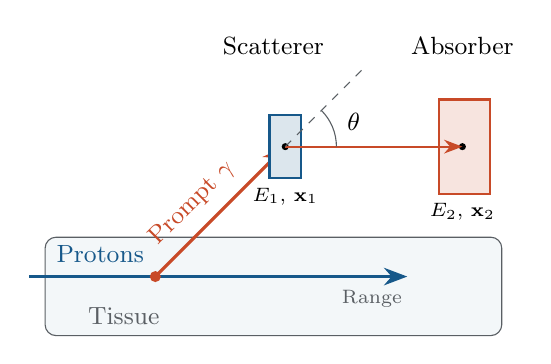
\begin{tikzpicture}[font=\small, >=Stealth]
        \filldraw[fill=crBlue!5,draw=crGrey,rounded corners]
          (0,0) rectangle (5.8,1.25);
        \node[crGrey] at (1.0,0.25) {Tissue};
        \draw[->,very thick,crBlue] (-0.2,0.75) -- (4.6,0.75);
        \node[above,crBlue] at (0.7,0.8) {Protons};
        \node[below,crGrey,font=\scriptsize] at (4.15,0.7) {Range};
        \fill[crRed] (1.4,0.75) circle (0.07);
        \draw[->,very thick,crRed] (1.4,0.75) -- (3.05,2.4);
        \node[rotate=45,above,crRed] at (2.05,1.5) {Prompt $\gamma$};
        \filldraw[fill=crBlue!15,draw=crBlue,thick]
          (2.85,2.0) rectangle (3.25,2.8);
        \filldraw[fill=crRed!15,draw=crRed,thick]
          (5.0,1.8) rectangle (5.65,3.0);
        \fill (3.05,2.4) circle (0.045);
        \fill (5.3,2.4) circle (0.045);
        \draw[->,thick,crRed] (3.05,2.4) -- (5.3,2.4);
        \draw[dashed,crGrey] (3.05,2.4) -- (4.05,3.4);
        \draw[crGrey] (3.7,2.4) arc[start angle=0,end angle=45,radius=0.65];
        \node at (3.92,2.72) {$\theta$};
        \node[above,align=center] at (2.9,3.45) {Scatterer};
        \node[above,align=center] at (5.3,3.45) {Absorber};
        \node[below,font=\scriptsize] at (3.05,2.0) {$E_1,\,\mathbf{x}_1$};
        \node[below,font=\scriptsize] at (5.3,1.8) {$E_2,\,\mathbf{x}_2$};
      \end{tikzpicture}}\\[2mm]
      {\scriptsize\color{crGrey} One photon, two detector interactions:
       Compton scattering followed by absorption.}\\[3mm]
      {\tiny\color{crGrey}
       \href{https://doi.org/10.3389/fonc.2016.00080}
       {Hueso-Gonz\'alez et al., Front. Oncol. 6:80 (2016).}\\
       \href{https://arxiv.org/abs/2202.06556}
       {Hybrid in-beam PET and Compton imaging (2022).}}
    \end{column}
  \end{columns}
\end{frame}


\begin{frame}{PET and Compton imaging: complementary measurements}
\small
\renewcommand{\arraystretch}{1.22}
\begin{tabular}{@{}>{\raggedright\arraybackslash}p{0.16\textwidth}>{\raggedright\arraybackslash}p{0.38\textwidth}>{\raggedright\arraybackslash}p{0.38\textwidth}@{}}
\toprule
 & \textbf{Prompt gammas / Compton} & \textbf{Induced activity / PET}\\
\midrule
Signal & Single prompt $\gamma$ rays, several MeV & Pairs of 511\,keV annihilation photons\\
Timing & During beam delivery & In the proposed in-room scheme, shortly after irradiation\\
Information & Emission profile along the beam; comparison with expected range & Activity distribution; comparison with expected distal edge\\
Main limitation & Few useful multi-interaction events and beam-related background & Decay, biological washout and patient registration\\
\bottomrule
\end{tabular}
\par\vspace{5mm}
\textbf{DIPC proposed strategy:} Compton imaging for monitoring during irradiation, followed by an in-room PET measurement within minutes of beam stop. Combine both results to minimize systematic errors.
\end{frame}

\begin{frame}{CRYSP: PET with cryogenic cesium iodide}
\small
\begin{columns}[T,onlytextwidth]
\begin{column}{0.31\textwidth}
\centering
\textbf{Pure CsI at $\sim$100 K}
\par\vspace{2mm}
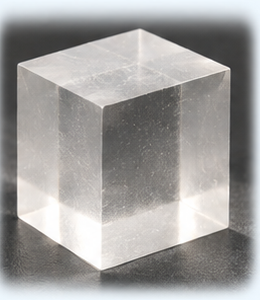
\includegraphics[height=0.27\textheight]{crysp_crystal.png}
\par\vspace{2mm}
\raggedright
\hi{$\sim10^5$ photons/MeV}.\\[2mm]
Abundant material; lower crystal cost than rare-earth scintillators.
\end{column}
\begin{column}{0.31\textwidth}
\centering
\textbf{Monolithic 3D detection}
\par\vspace{2mm}
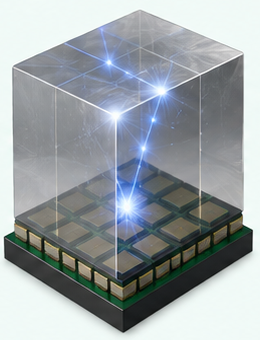
\includegraphics[height=0.27\textheight]{crysp_monolithic.png}
\par\vspace{2mm}
\raggedright
Large crystals read out by silicon photomultipliers (SiPMs).\\[2mm]
\hi{Millimetre-scale 3D resolution} in simulation; measured energy resolution \hi{below 7\%} at 511\,keV.
\end{column}
\begin{column}{0.31\textwidth}
\centering
\textbf{Full-ring PET}
\par\vspace{2mm}
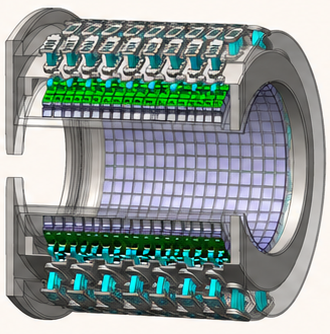
\includegraphics[height=0.27\textheight]{crysp_ring.png}
\par\vspace{2mm}
\raggedright
Total-body PET design based on these crystals.\\[2mm]
\hi{High sensitivity at lower detector cost} is the design goal.
\end{column}
\end{columns}
\source{https://doi.org/10.1088/1361-6560/ae35c8}{R. Soleti, J.J. Gomez-Cadenas et al., Phys. Med. Biol. 71, 025001 (2026).}
\end{frame}

\begin{frame}{COCOA: a compact Compton camera for MeV gamma rays}
\small
\begin{columns}[T,onlytextwidth]
\begin{column}{0.31\textwidth}
\centering
\textbf{LiquidO scatterer}
\par\vspace{2mm}
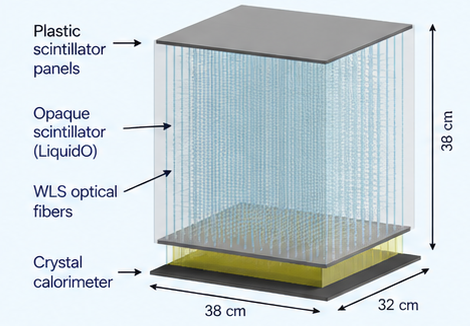
\includegraphics[width=\linewidth,height=0.27\textheight,keepaspectratio]{cocoa_scatterer.png}
\par\vspace{2mm}
\raggedright
Opaque liquid scintillator with a 3D grid of wavelength-shifting fibres.\\[2mm]
Reconstructs the \hi{position and energy} of the first interaction.
\end{column}
\begin{column}{0.31\textwidth}
\centering
\textbf{Crystal absorber}
\par\vspace{2mm}
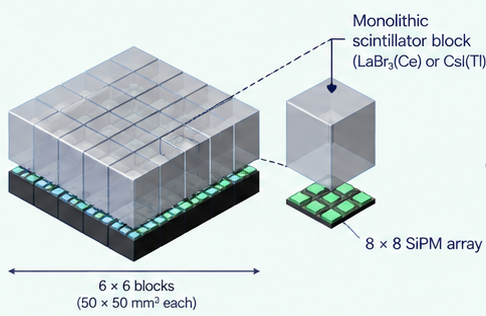
\includegraphics[width=\linewidth,height=0.27\textheight,keepaspectratio]{cocoa_absorber.png}
\par\vspace{2mm}
\raggedright
Monolithic scintillator blocks read out by SiPM arrays.\\[2mm]
Measures the scattered photon: \hi{3D position and energy}, including depth of interaction.
\end{column}
\begin{column}{0.31\textwidth}
\centering
\textbf{Space application}
\par\vspace{2mm}
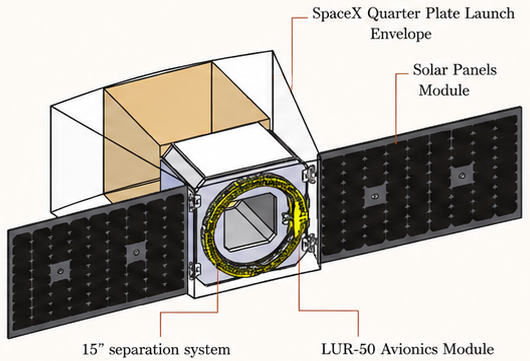
\includegraphics[width=\linewidth,height=0.27\textheight,keepaspectratio]{cocoa_satellite.png}
\par\vspace{2mm}
\raggedright
Designed for \hi{MeV gamma-ray astronomy}.\\[2mm]
Compact geometry for microsatellites or high-altitude balloons; proposed LUR-50 integration shown.
\end{column}
\end{columns}
\source{https://doi.org/10.1016/j.astropartphys.2025.103135}{R. Soleti, J.J. Gomez-Cadenas et al., Astropart. Phys. 172, 103135 (2025).}
\end{frame}

\begin{frame}{CRYSP: \emph{CRYogenic Sensitive PET}}
  \begin{columns}[T]
    \begin{column}{0.6\textwidth}
      \begin{itemize}
        \item Scintillators \hi{CsI and BGO} gain dramatically in light yield
          when cooled --- at 77 K, CsI reaches $\sim$100 photons/keV and BGO
          $\sim$29 photons/keV.
            \item In both cases, high yields translate into excellent energy resolution
              (6\% CsI, 10\% BGO),
              which in turn is essential for efficient scatter rejection.
        \item Monolithic crystals + SiPMs permit 3D position reconstruction using neural
              networks with high accuracy and no parallax error.
      \end{itemize}

    \end{column}
    \begin{column}{0.4\textwidth}
      \centering
      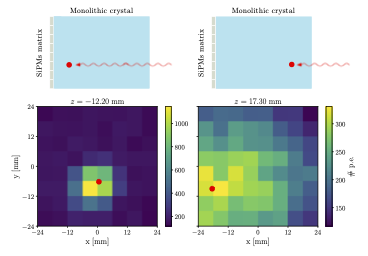
\includegraphics[width=\linewidth]{3D.png}\\
      {\scriptsize\color{crGrey} 3D reconstruction in a monolithic crystal.}
    \end{column}
  \end{columns}
\end{frame}

\begin{frame}{Scanner cost breakdown}
  \centering
  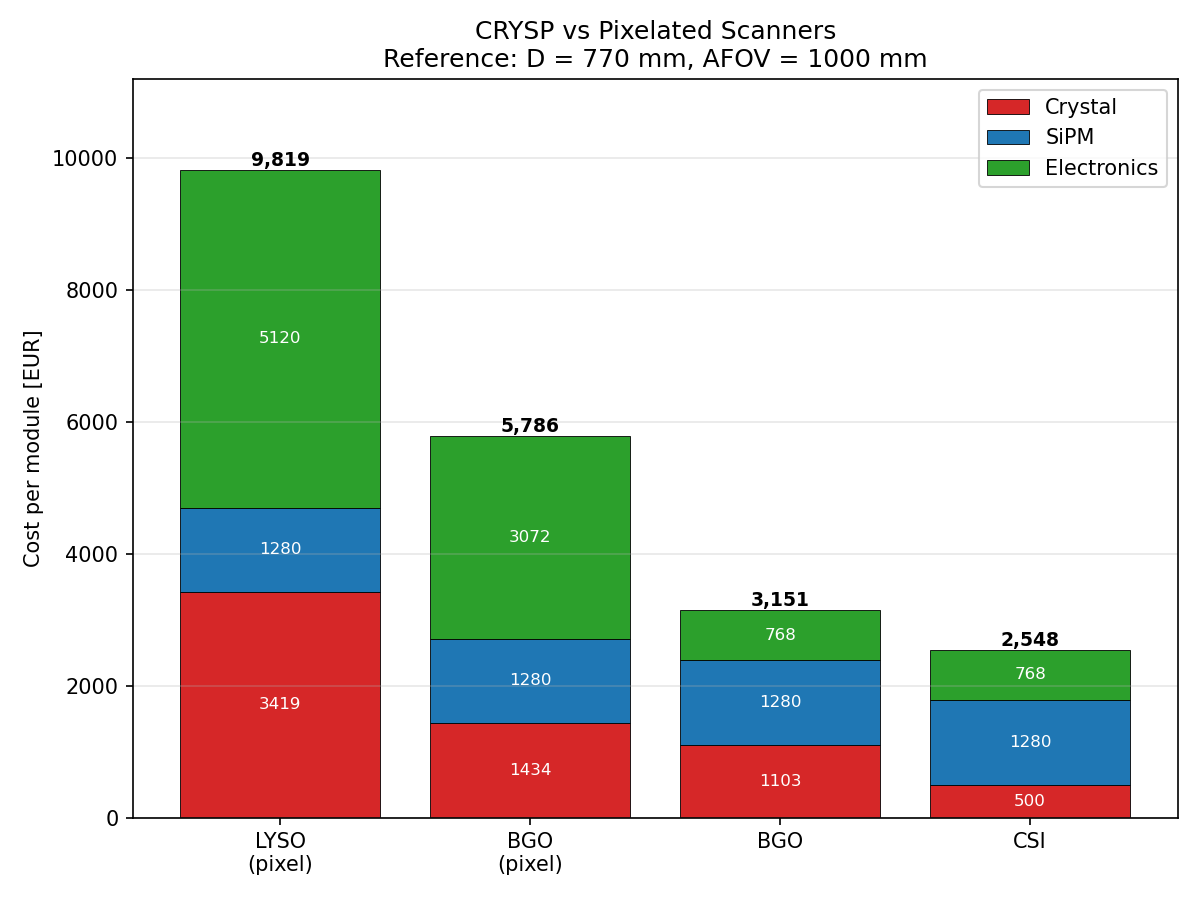
\includegraphics[width=0.94\textwidth,height=0.80\textheight,keepaspectratio]{cost_breakdown.png}
\end{frame}

\begin{frame}{Total scanner cost}
  \centering
  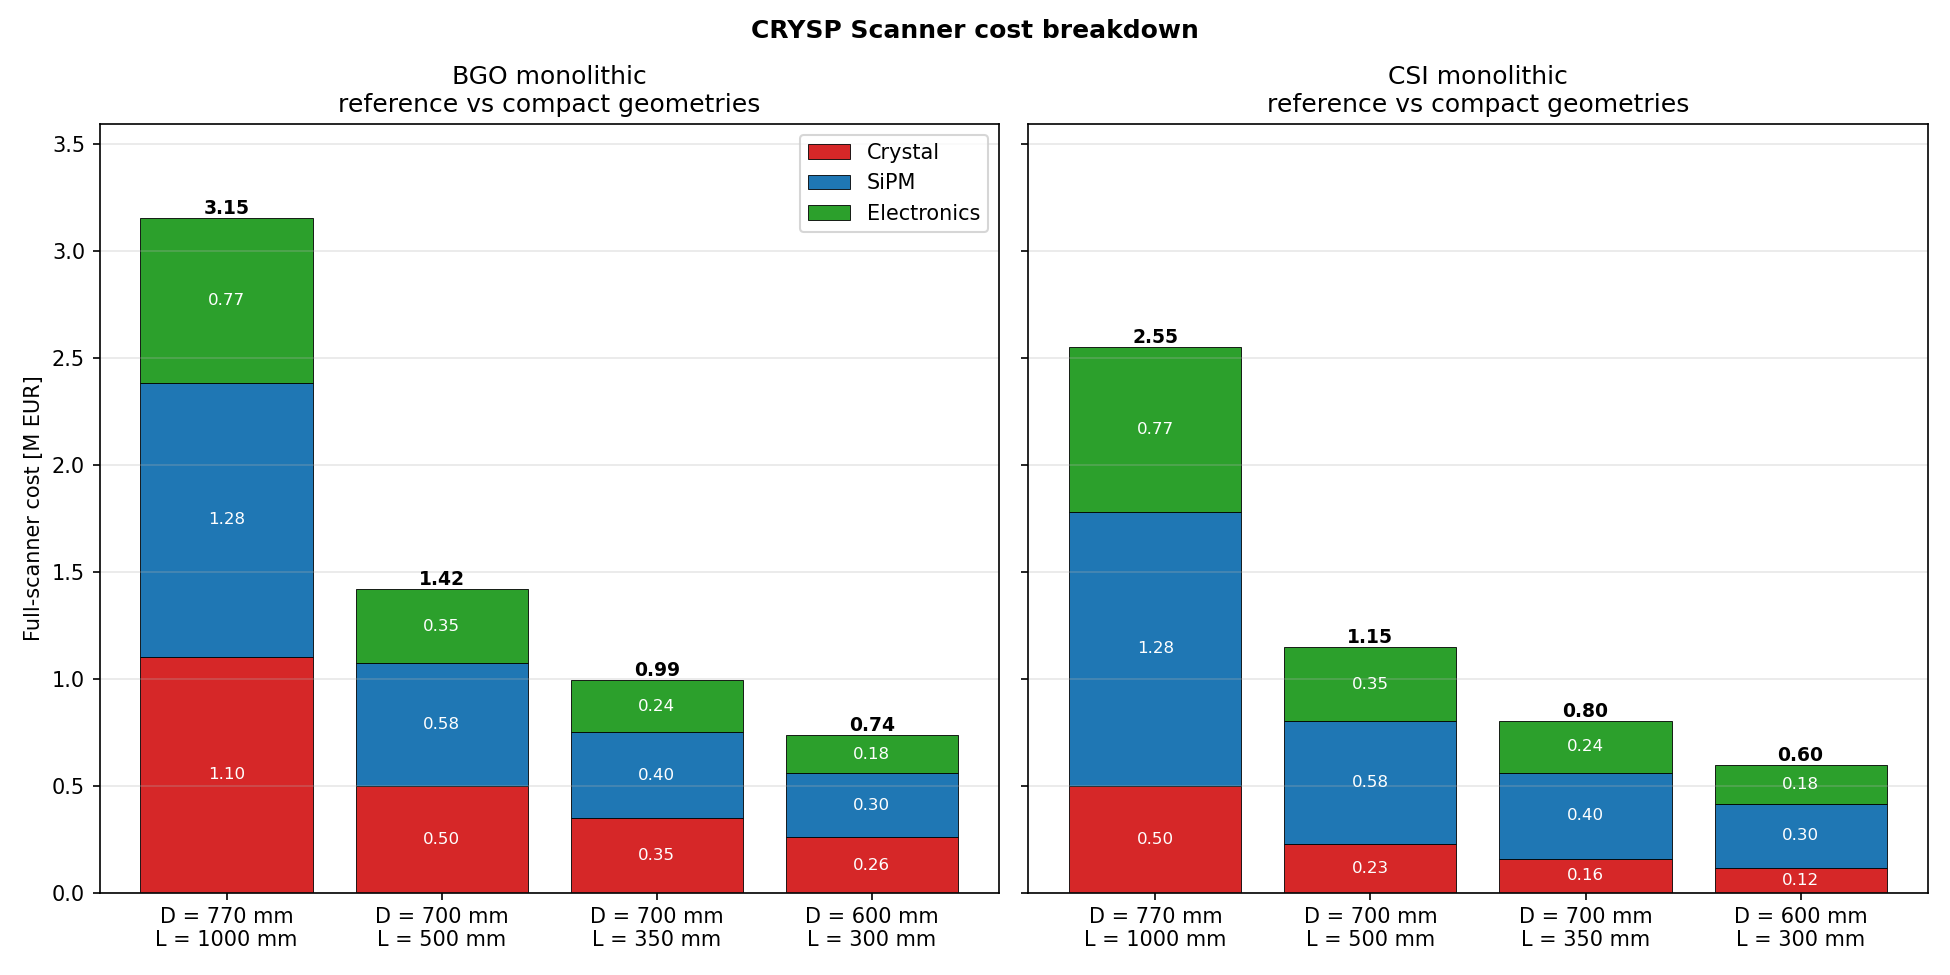
\includegraphics[width=0.94\textwidth,height=0.80\textheight,keepaspectratio]{scanner_totals.png}
\end{frame}

\begin{frame}{Reference protocol: all scanner configurations are sub-mm}
  \begin{columns}[T]
    \begin{column}{0.44\textwidth}
      \begin{itemize}
        \item \hi{Protocol:} 1\,Gy, 300\,s acquisition, starting 120\,s after
          beam-off; washout included.
        \item BGO: \hi{0.101--0.127\,mm}; CsI: \hi{0.146--0.155\,mm}.
        \item BGO is more precise through higher sensitivity; CsI remains a
          competitive, lower-cost option.
        \item These values are the \hi{statistical precision of the fitted
          activity edge}.
      \end{itemize}
    \end{column}
    \begin{column}{0.56\textwidth}
      \centering
      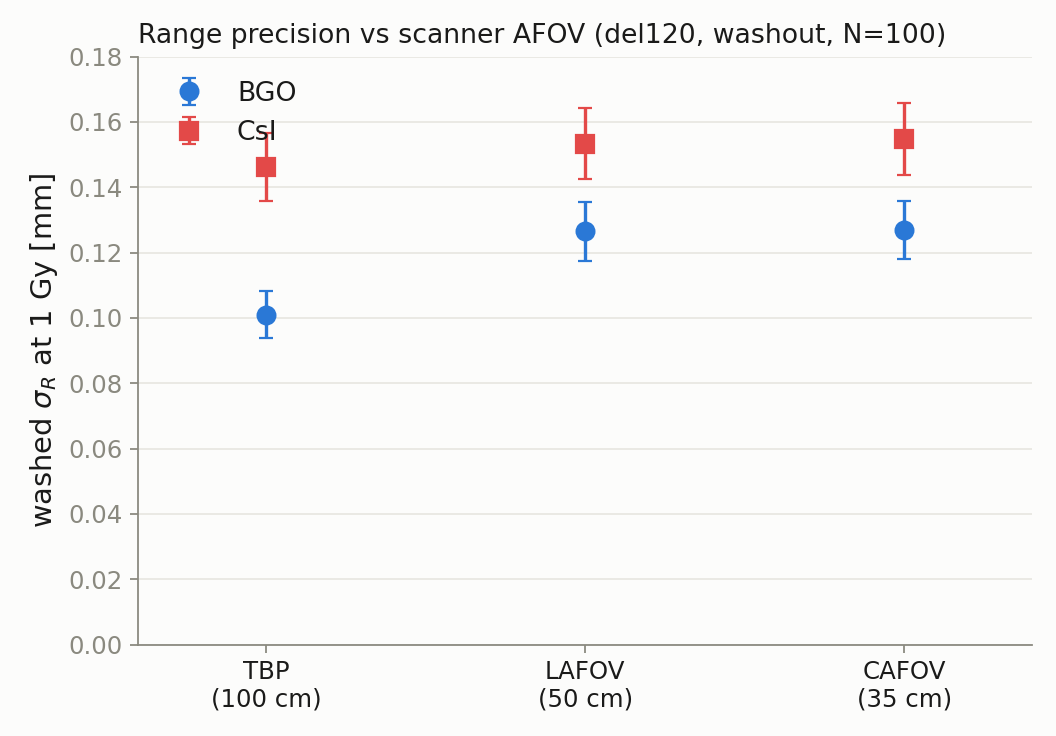
\includegraphics[width=\linewidth]{statproc_washed_grid.png}\\
      {\scriptsize\color{crGrey} Finite-pool-corrected $\sigma_R$ for the
       reference protocol ($N=100$).}
    \end{column}
  \end{columns}
\end{frame}

% \begin{frame}{Summary}
%   \begin{itemize}
%     \item Proton-therapy range verification needs an \hi{in vivo}, online/in-room,
%       high-sensitivity probe
%     \item \hi{CRYSP in-room PET} exploits cryogenic CsI/BGO for excellent energy
%       and spatial resolution at a \hi{competitive cost}.
%     \item For the reference protocol, the fitted activity edge has
%       \hi{0.101--0.155\,mm statistical precision} across all BGO and CsI
%       geometries; the tested CsI timing grid remains below 0.35\,mm.
%     \item CsI offers a very good, low-cost, supply-secure option; BGO offers
%       the best statistical precision.
%   \end{itemize}
%   \vspace{3mm}
% \end{frame}

\begin{frame}{Proton therapy: worldwide deployment and growth in Europe}
\small
\begin{columns}[T,onlytextwidth]
\begin{column}{0.59\textwidth}
\centering
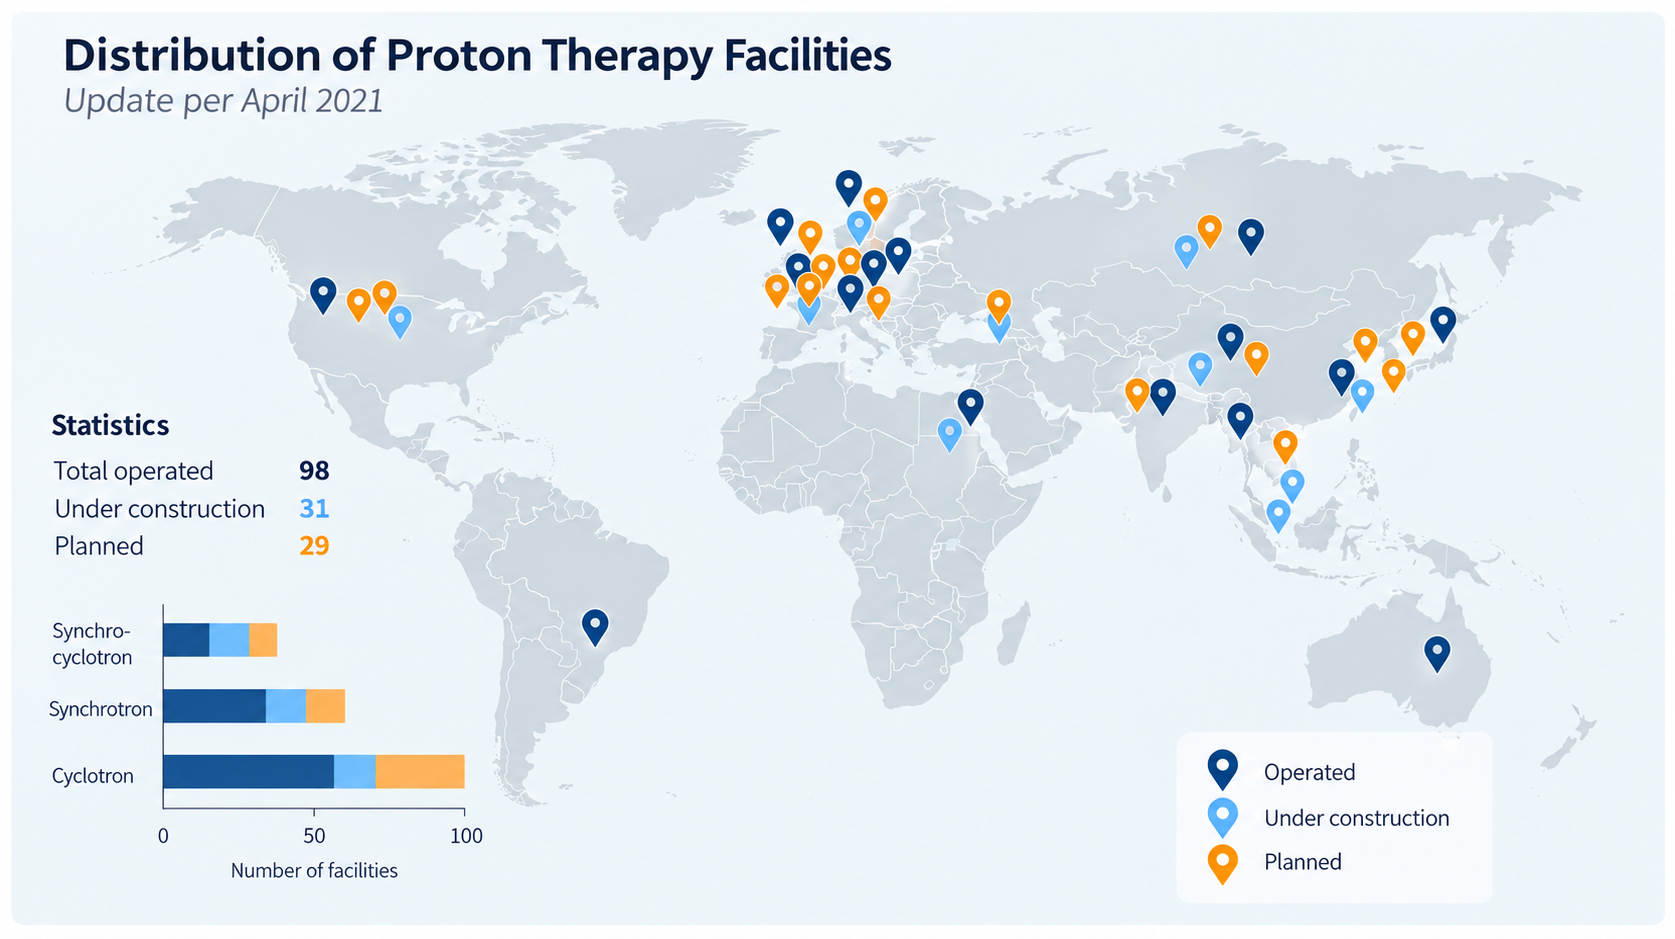
\includegraphics[width=\linewidth]{proton_facilities_world_2021.png}
\par\vspace{2mm}
\raggedright
Over the last two decades, proton therapy has evolved from a highly specialised treatment into a \hi{globally deployed clinical technology}.
\end{column}
\begin{column}{0.38\textwidth}
\centering
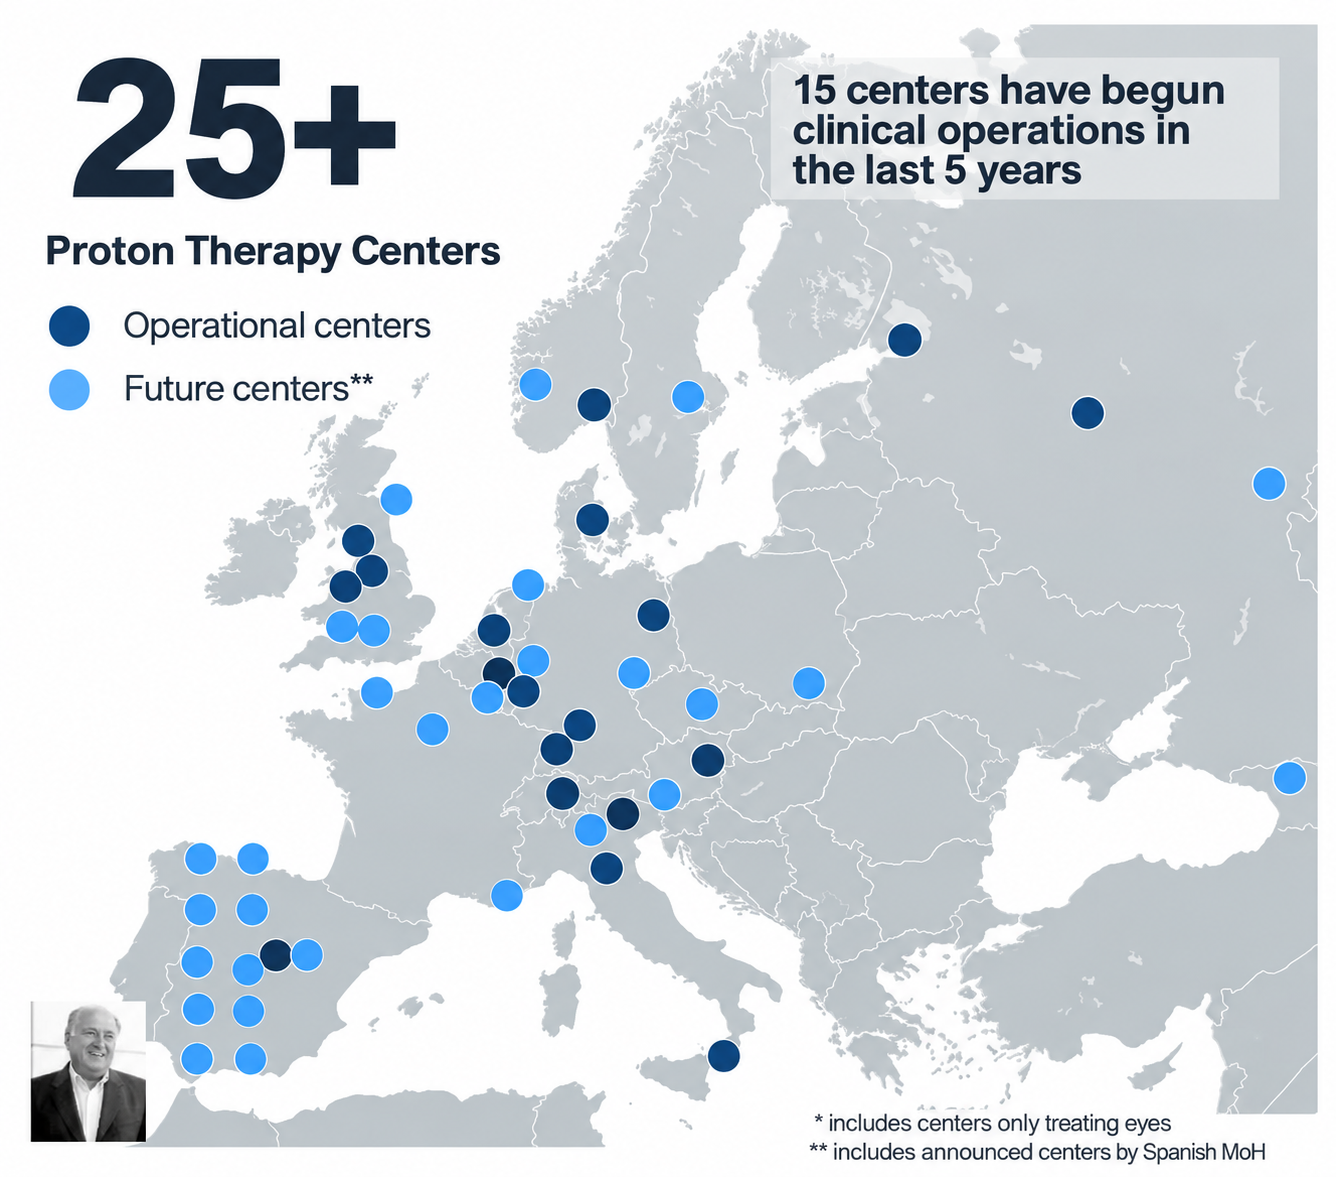
\includegraphics[height=0.33\textheight,keepaspectratio]{proton_facilities_europe.png}
\par\vspace{2mm}
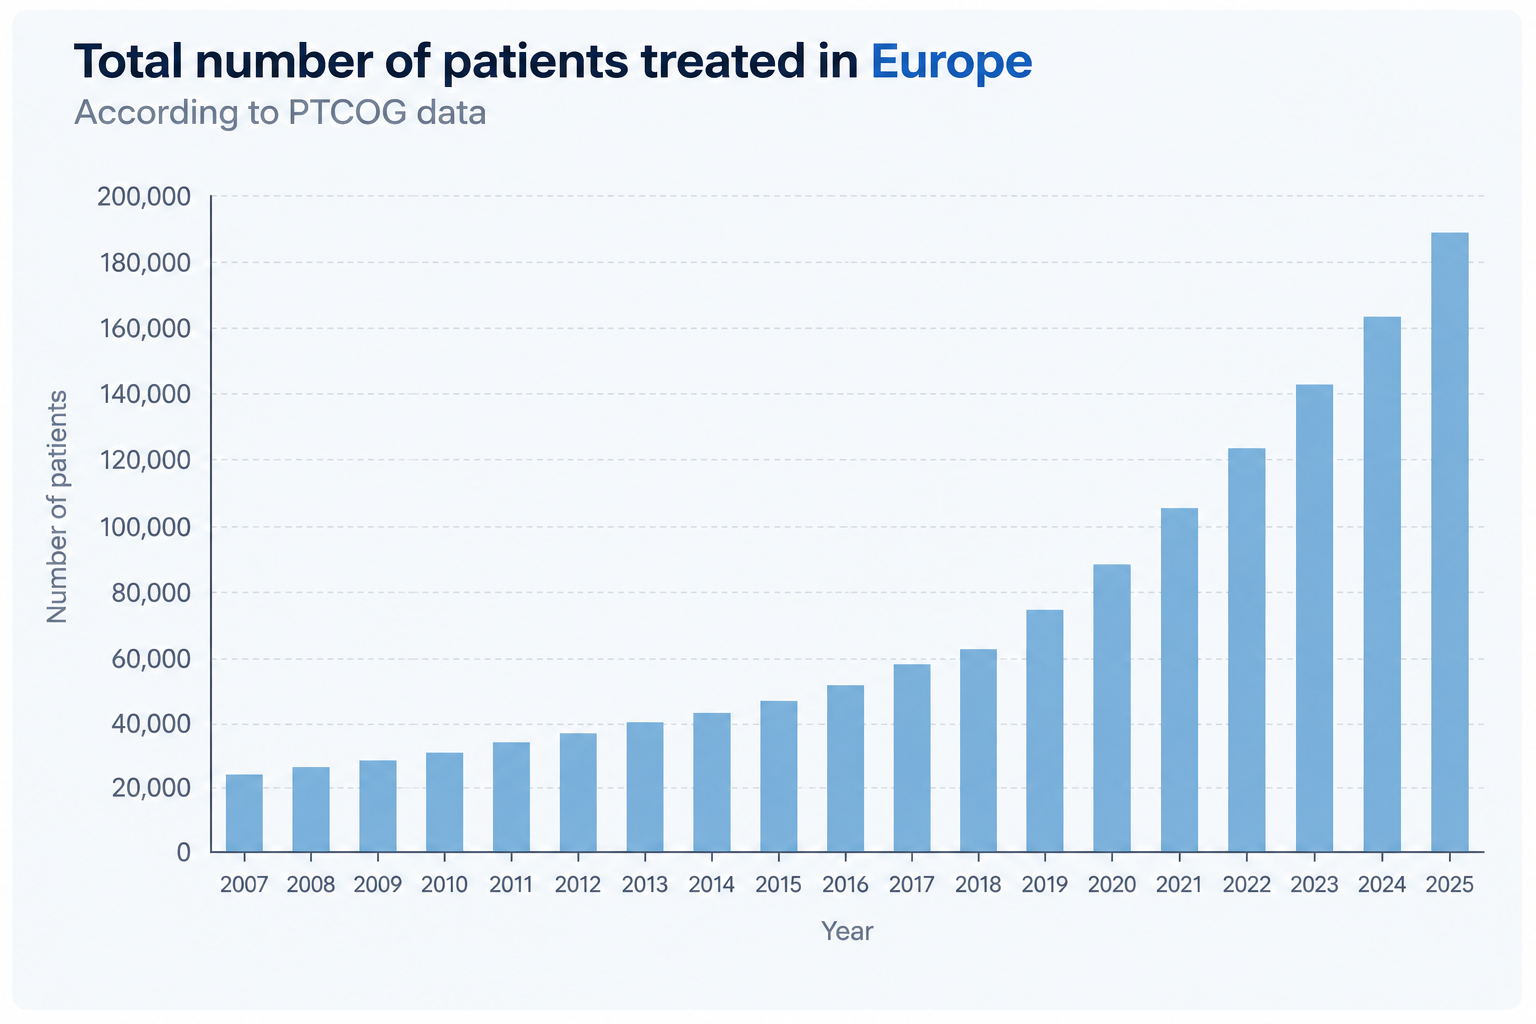
\includegraphics[width=\linewidth,height=0.33\textheight,keepaspectratio]{proton_patients_europe.png}
\end{column}
\end{columns}
\par\vspace{2mm}
{\tiny\color{crGrey} World map: April 2021. European patient chart: PTCOG attribution in the supplied figure; numerical series not independently verified.}
\end{frame}

\begin{frame}{Clinical evidence for proton therapy}
\small
\begin{columns}[T,onlytextwidth]
\begin{column}{0.49\textwidth}
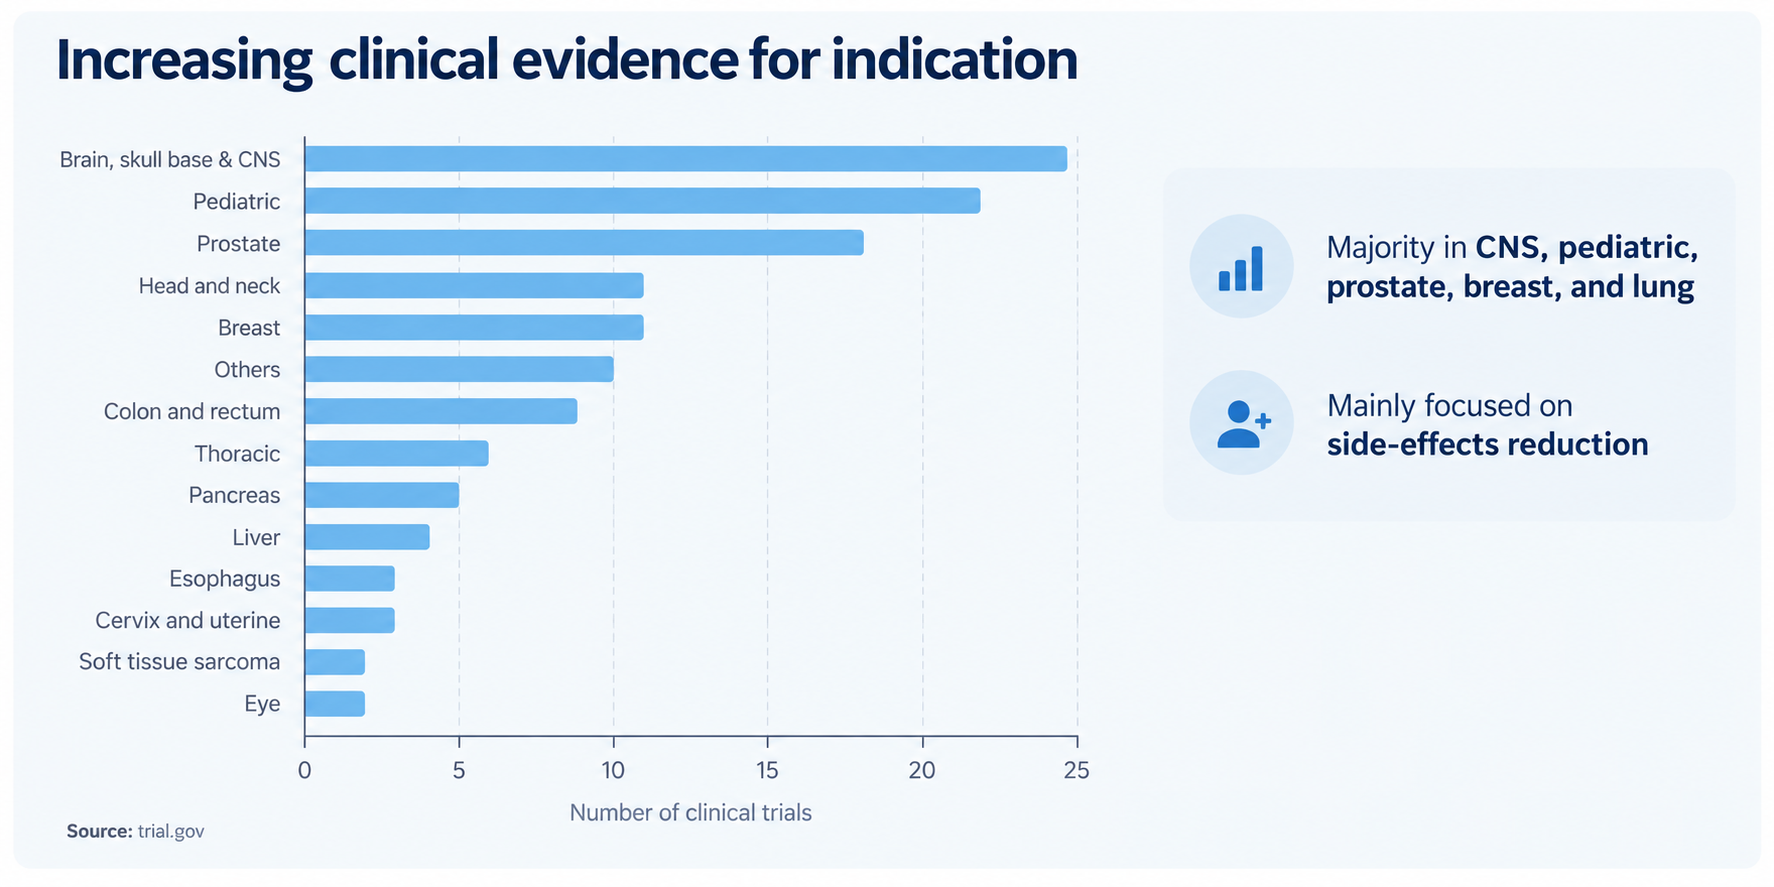
\includegraphics[width=\linewidth]{proton_trials_indications.png}
\end{column}
\begin{column}{0.49\textwidth}
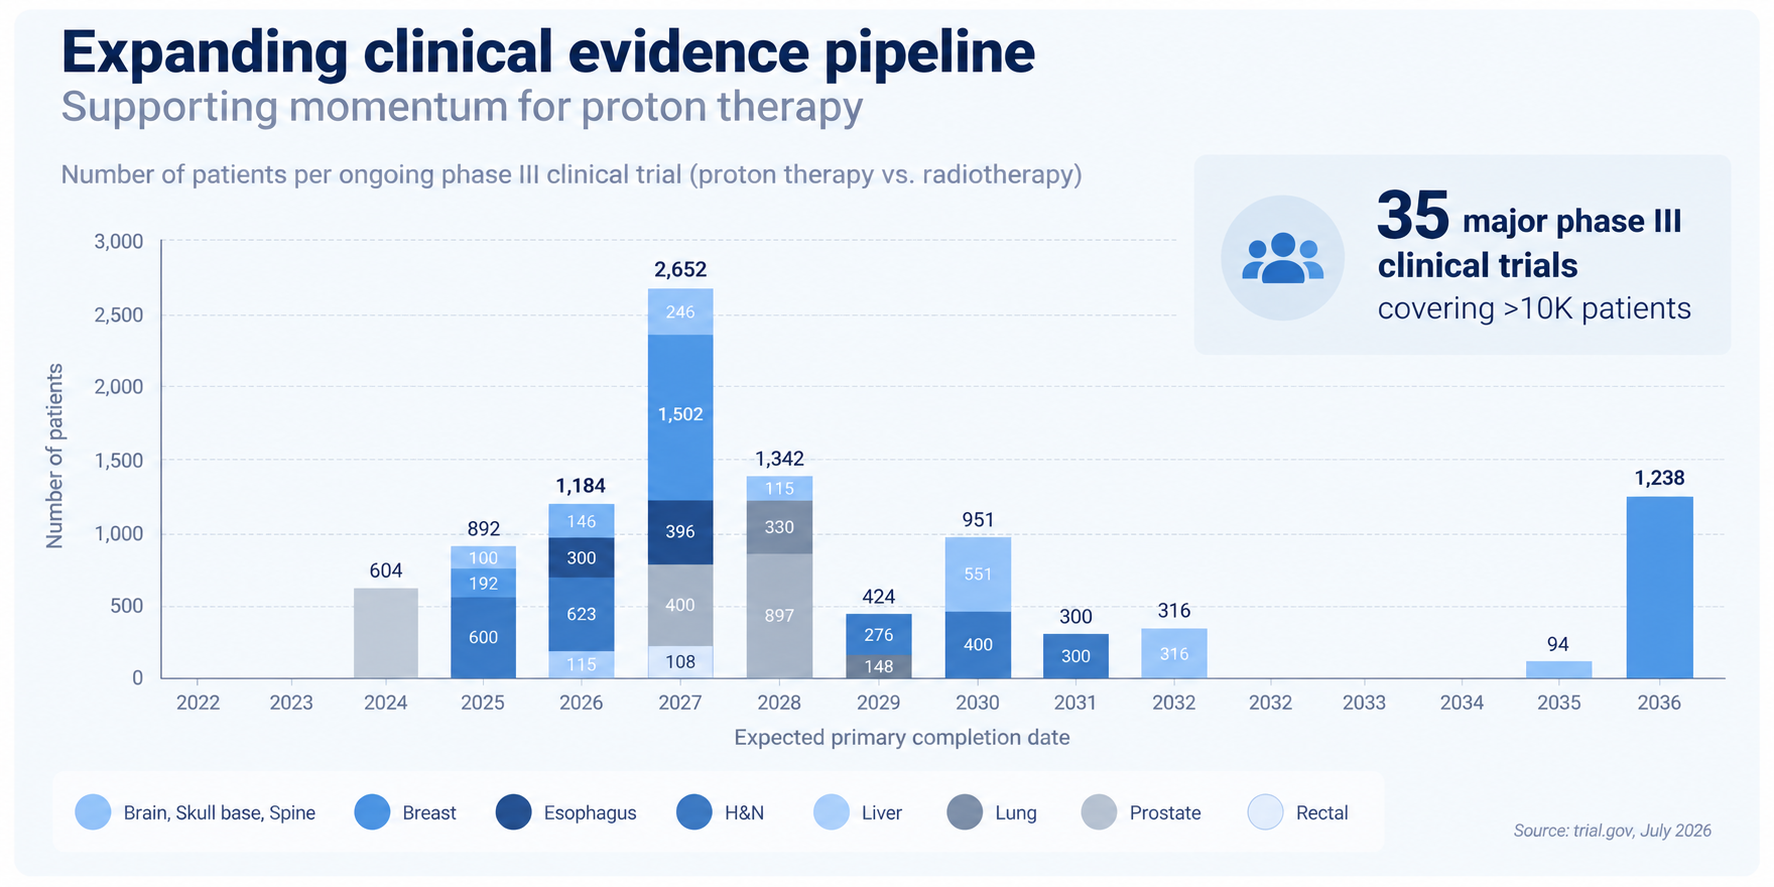
\includegraphics[width=\linewidth]{proton_trials_phase3.png}
\end{column}
\end{columns}
\par\vspace{5mm}
\raggedright
Phase III trials are building the \hi{clinical evidence} for wider use of proton therapy, particularly to \hi{reduce side effects}.
\par\vspace{1mm}
{\tiny\color{crGrey} Supplied charts cite trial.gov (phase III chart: July 2026). Trial counts and projected completion dates require registry verification.}
\end{frame}

\begin{frame}{Boosting proton therapy}
\small
\begin{enumerate}
\item Proton beam dose monitoring \hi{in real time} is a real need that will become more pressing as the number of centres grows and the number of treated patients increases.
\item R\&D on monitoring techniques has been going on for about 20 years. PET and gamma cameras offer the potential for \hi{day-by-day, case-by-case monitoring} and distal-edge measurements that could reduce underdose while minimising the risk of overdose.
\item However, these systems have \hi{not yet become standard medical practice}.
\end{enumerate}
\source{https://doi.org/10.3389/fonc.2025.1660605}{Clinical status: Current status and upcoming developments for online adaptive proton therapy, Front. Oncol. (2025).}
\end{frame}

\begin{frame}{The DIPC group}
\small
The DIPC group is a leading neutrino physics group in Spain, with extensive expertise in \hi{nuclear instrumentation}.
\par\vspace{2mm}
\begin{columns}[T,onlytextwidth]
\begin{column}{0.49\textwidth}
\textbf{Scientific leadership and concepts}
\begin{itemize}
\item Led by \hi{J.J. Gomez-Cadenas}: co-recipient of the \hi{2016 Breakthrough Prize in Fundamental Physics} as a member of K2K and T2K, with group leadership roles in neutrino physics.
\item Two ERC grants: \hi{AdG-2013 and SyG-2020}.
\item \hi{CRYSP}: Gomez-Cadenas, Soleti, Lopez-Guejo, Pelegrin.\\
\hi{COCOA}: Soleti, Gomez-Cadenas.
\end{itemize}
\end{column}
\begin{column}{0.49\textwidth}
\textbf{Team, engineering and management}
\begin{itemize}
\item Four faculty, two engineers, two postdocs, and graduate and undergraduate students.
\item Substantial experience in mechanical engineering and cryogenics.
\item Strong Basque industry connections and established management: Lopez-Guejo and Pelegrin.
\item Well funded by the ERC and Basque Government; additional positions planned for CRYSP and COCOA.
\end{itemize}
\end{column}
\end{columns}
\end{frame}

\begin{frame}{CRYSP and COCOA for proton beam monitoring}
\small
\begin{itemize}
\item The CRYSP and COCOA concepts can be applied as \hi{high-performance, low-cost solutions} for proton beam monitoring. Our recent study shows the potential of in-room CRYSP PET.
\item We have \hi{operating prototypes of both systems} and are moving towards the construction of larger apparatus.
\item The group is establishing a close collaboration with \hi{Biogipuzkoa} and the medical staff of the forthcoming proton beam therapy centre in \hi{Donostia}.
\end{itemize}
\par\vspace{3mm}
{\scriptsize\color{crGrey} J.J. Gomez-Cadenas et al., \emph{A High-Sensitivity In-Room CRYSP Scanner for Distal-Edge Verification in Proton Therapy}, paper in preparation, available upon request.}
\end{frame}

\begin{frame}{Our vision: an integrated monitoring service}
\small
\begin{itemize}
\item Optimised, \hi{high-precision, low-cost apparatus}, combined with fast and efficient software using \hi{AI-enabled technologies}, to provide real-time monitoring and support treatment correction in cooperation with doctors.
\item A potential spin-off, \hi{ARGOS}, would offer an integrated solution to proton therapy centres:
\end{itemize}
\par\vspace{2mm}
\begin{columns}[T,onlytextwidth]
\begin{column}{0.31\textwidth}
\centering\textbf{Hardware}\\[2mm]
Installation and maintenance
\end{column}
\begin{column}{0.31\textwidth}
\centering\textbf{Software}\\[2mm]
Full development and integration
\end{column}
\begin{column}{0.31\textwidth}
\centering\textbf{Day-by-day service}\\[2mm]
Close cooperation with doctors
\end{column}
\end{columns}
\par\vspace{5mm}
The model could be extensively tested and optimised in \hi{Donostia}, then expanded to new proton beam centres.
\end{frame}

\begin{frame}{Development programme and investment}
\small
\textbf{Foreseen development cycle: \hi{3--4 years}.}
\par\vspace{3mm}
\textbf{Investment: approximately \hi{\euro1 million per year}, or \hi{\euro3--4 million in total}.}
\par\vspace{5mm}
\begin{enumerate}
\item Validation of prototypes.
\item Preclinical demonstrators.
\item Clinical trials and medical validation.
\item Construction of medical-grade apparatus.
\item Initial operation.
\end{enumerate}
\end{frame}

\end{document}
